\section{Experiment}


\begin{table*}[t]
\centering
\caption{Out-of-distribution comparison on held-out datasets, including generalization capability and performance on unseen classes. Values represent mean Dice scores (\%). All in-context models use one-shot inference.}
\label{tab:ood_results}
%\definecolor{lightgray}{rgb}{0.92, 0.92, 0.92}
\setlength{\tabcolsep}{1.4em}
\resizebox{0.9\textwidth}{!}{ %\columnwidth
\begin{tabular}{l|ccccc|cc}
\toprule
\multirow{2}{*}{Method} & \multicolumn{5}{c|}{Generalization} & \multicolumn{2}{c}{Unseen Classes} \\
\cline{2-8}
& ACDC & SegTHOR & CSI-inn & CSI-opp & CSI-fat & MSD Pancreas & Pelvic \\
\midrule
\multicolumn{8}{l}{\textit{Supervised Upper Bound}} \\
nnUNet & 90.97 & 89.78 & 91.23 & 91.04 & 90.13 & 54.56 & 94.73 \\
\midrule
\multicolumn{8}{l}{\textit{Task-specific Model}} \\
nnUNet-generalize & 82.06 & 76.92 & 55.24 & 85.19 & 0.23 & -- & -- \\
\midrule
\multicolumn{8}{l}{\textit{Multi-task Universal Model}} \\
CLIP-driven & 84.72 & 78.23 & 59.73 & 86.73 & 1.47 & -- & -- \\
UniSeg & 84.98 & 78.56 & 60.02 & 86.13 & 1.52 & -- & -- \\
Multi-Talent & 83.79 & 78.45 & 58.29 & 87.01 & 1.95 & -- & -- \\
\midrule
\multicolumn{8}{l}{\textit{Positional Prompt}} \\
SAM-Med2D & 42.23 & 52.37 & 29.23 & 32.71 & 10.91 & 10.37 & 35.71 \\
SAM-Med3D & 51.49 & 68.97 & 45.32 & 68.72 & 23.93 & 15.83 & 53.61 \\
\midrule
\multicolumn{8}{l}{\textit{In-context}} \\
SegGPT & 73.82 & 60.98 & 59.87 & 77.62 & 35.27 & 10.67 & 55.92 \\
UniverSeg & 72.43 & 54.75 & 63.48 & 85.32 & 52.48 & 10.28 & 57.81 \\
Tyche-IS & 74.91 & 56.75 & 64.23 & 87.13 & \textbf{55.75} & 11.97 & 61.92 \\
\rowcolor{lightgray} Iris (ours) & \textbf{86.45} & \textbf{82.77} & \textbf{64.44} & \textbf{89.13} & 47.78 & \textbf{28.28} & \textbf{69.03} \\
\bottomrule
\end{tabular}
}
\vspace{-1em}
\end{table*}



\subsection{Experimental Setup}
We evaluate Iris across three key dimensions: in-distribution performance on trained tasks, out-of-distribution generalization to different domains, and adaptability to novel anatomical classes. Additional experiments analyze Iris's computational efficiency, inference strategies, and architectural design choices.

\noindent\textbf{Dataset.}
Our training data comprises 12 public datasets~\cite{bcv,bilic2019liver,heller2019kits19,ji2022amos,structseg,CHAOS2021,campello2021multi,rodrigue2012beta,gatidis2022whole,martin2023deep} spanning diverse body regions (head, chest, abdomen), modalities (CT, MRI, PET), and clinical targets (organs, tissues, lesions), split into 75\%/5\%/20\% for train/validation/test. For out-of-distribution evaluation, we use 5 held-out datasets: ACDC~\cite{bernard2018deep}, SegTHOR~\cite{lambert2020segthor}, and three MRI modalities from IVDM3Seg~\cite{ivdm3seg} to evaluate robustness against domain shift; MSD Pancreas (Tumor)~\cite{antonelli2022medical} and Pelvic1K (Bone)~\cite{liu2021deep} datasets are used for novel class adaptation. We randomly select 20\% samples from held-out sets for testing. Detailed dataset information is provided in supplementary materials.

\noindent\textbf{Baseline Models.} 
We compare against four categories of methods:
(1) Task-specific models: nnUNet~\cite{isensee2021nnu};
(2) Universal models: CLIP-driven model~\cite{liu2023clip}, UniSeg~\cite{ye2023uniseg} and Multi-Talent~\cite{ulrich2023multitalent};
(3) Foundation models: SAM~\cite{kirillov2023segment} and its medical variants, SAM-Med2D~\cite{cheng2023sam}, SAM-Med3D~\cite{wang2024sam};
(4) In-context learning methods: SegGPT~\cite{wang2023seggpt}, UniverSeg~\cite{butoi2023universeg}, and Tyche-IS~\cite{rakic2024tyche}.
All models are trained on our curated dataset, except SAM, with 2D models trained on extracted slices and 3D models with 3D volumes. For SAM-based methods, we simulate user interactions using ground-truth labels during training and evaluation.

\noindent\textbf{Implementation Details.}
Iris uses a 3D UNet encoder trained from scratch with one-shot learning strategy. We employ the Lamb optimizer~\cite{you2019large} with exponential learning rate decay (base lr=$2\times10^{-3}$, weight decay=$1\times10^{-5}$), training for 80K iterations with batch size 32 and 2K warm-up iterations. Data augmentation includes random cropping, affine transformations, and intensity adjustments. Training and inference use $128\times128\times128$ volume size.


\subsection{Comparison with the state-of-the-art}

\noindent\textbf{Results on in-distribution classes.}
We evaluate Iris's performance on twelve diverse medical datasets used during training. As shown in Table \ref{tab:id_results}, Iris achieves state-of-the-art performance with an average Dice score of 84.52\%, matching or exceeding task-specific and multi-task models that are optimized for fixed tasks.
Existing adaptive approaches show significant limitations. SAM-based methods perform poorly due to their strong reliance on simple positional prompts, with the large performance gap between their 2D and 3D variants (40.58\% vs. 68.42\%) highlighting the importance of 3D context. Existing in-context learning methods, like SegGPT, UniverSeg, (best: 61.20\%) struggle particularly with 3D tasks like AMOS and LiTS due to their 2D architecture, though performing better on 2D-friendly tasks like MnM and CSI-Wat. In contrast, Iris's 3D architecture and efficient task encoding enables consistent high-level performance across all tasks while maintaining its adaptability to unseen novel anatomical classes.







\noindent\textbf{Results on OOD generalization.} We evaluate out-of-distribution (OOD) performance on five held-out datasets spanning two types of distribution shifts: cross-center variation (ACDC, SegTHOR) and cross-modality adaptation (CSI variants). In Table \ref{tab:ood_results}, Iris demonstrates superior performance across all scenarios, particularly excelling in challenging 3D tasks and large domain shifts.

Both task-specific and multi-task universal models show performance degradation, especially failing catastrophically on CSI-fat with a significant domain gap. While SAM-based methods demonstrate their resilience to domain shifts through strong prior knowledge injected from user interactions, their performance remains limited on the volumetric data.
In-context learning methods retain a good performance with cross-modality adaptation (e.g. on CSI-fat), benefiting from the domain-specific knowledge provided by reference examples. However, a 2D-slice-based architecture (e.g., UniverSeg and Tyche) limits its capability on 3D tasks like SegTHOR. In contrast, Iris's task encoding module efficiently extracts and utilizes 3D domain-specific information from the reference examples. 


\noindent\textbf{Results on novel classes.} To measure the adaptation performance to completely unseen anatomical structures, we evaluate on MSD Pancreas Tumor and Pelvic datasets. Using only one reference example, Iris achieves 28.28\% on MSD Pancreas Tumor and 69.03\% on Pelvic segmentation, substantially outperforming other adaptive methods (the best competitor: 11.97\% and 61.92\% respectively). This performance gain is particularly notable given that traditional task-specific models and multi-task models can not handle these novel classes without retraining. These findings demonstrate Iris's strong capability in learning from very limited examples while maintaining meaningful segmentation quality on previously unseen anatomical structures.




\noindent\textbf{Efficiency comparison}
 We analyze computational efficiency for segmenting $m$ query images with $n$ classes using $k$ reference pairs. Iris achieves superior efficiency through two key designs: decoupling task extraction from inference and handling multiple classes in a single forward pass. This results in complexity of $O(k + m)$ compared to $O(kmn)$ in methods like UniverSeg that process each class separately and recompute reference features for every query.

Table~\ref{tab:complexity} compares real-world inference time and memory usage across methods. While UniverSeg's slice-by-slice processing leads to significant overhead with multiple reference slices, and SAM-Med3D requires iterative user interactions (interaction-time not included), Iris efficiently processes entire 3D volumes all at once. For a scenario of segmenting 10 query volumes with 15 classes using one reference volume, Iris completes in 2 seconds. This efficiency advantage grows with more context examples due to Iris's decoupled architecture eliminating redundant reference processing.

\begin{table}[t]
\centering
\caption{Comparison of computational complexity. Empirical measurements of computation on one NVIDIA A100 GPU. We inference with 10 query images and one reference image from AMOS CT dataset with 15 classes. The image size is processed to $128\times128\times128$ for inference.}
\label{tab:complexity}
\resizebox{0.9\columnwidth}{!}{
\begin{tabular}{lccc}
\toprule
Method & Inference Time (s) & Memory (GB) & Parameters (M) \\
\midrule
UniverSeg-1 & 659.4 & 2.1 & 1.2 \\
UniverSeg-128 & 1030.2 & 12.1 & 1.2 \\
SAM-Med2D & 648.4 & 1.8 & 91.1 \\
SAM-Med3D & 15.2 & 2.9& 100.5 \\
\rowcolor{lightgray}Iris (Ours) & 2.0 & 7.4 & 69.4 \\
\bottomrule
\end{tabular}
}
\vspace{-1em}
\end{table}



\subsection{Analysis}


\begin{figure}[t]
\begin{center}
%\framebox[4.0in]{$\;$}
%\fbox{\rule[-.5cm]{0cm}{4cm} \rule[-.5cm]{4cm}{0cm}}
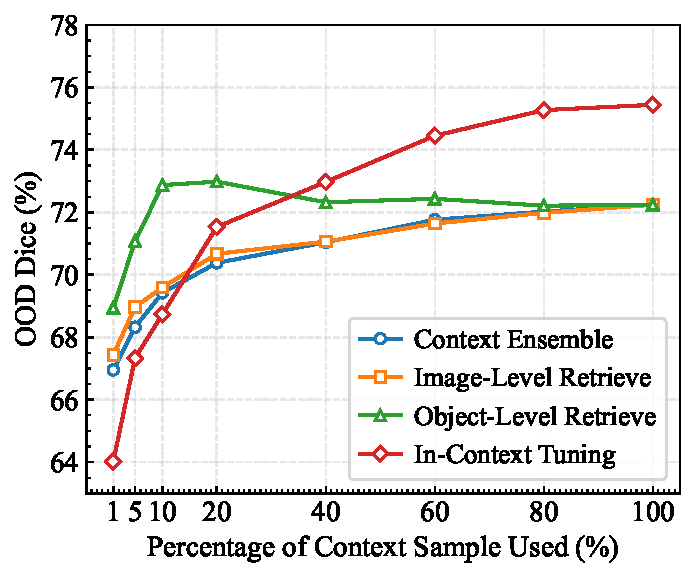
\includegraphics[width=0.7\columnwidth]{./fig/inference_comparison.pdf}
\end{center}
\vspace{-1em}
\caption{Analysis of different inference strategies.}
\label{fig:inference_comparison}
\vspace{-1em}
\end{figure}

\noindent\textbf{Inference strategy.} Figure~\ref{fig:inference_comparison} compares our four inference strategies. In this experiment, we maintain a pool of all available context examples and evaluate each strategy's performance as follows.

Context ensemble randomly selects and averages task embeddings from a percentage of the context pool. When using only one context example (1\%), it operates as one-shot inference. Performance of context ensemble keeps improving with more context examples and eventually saturates. This strategy is appealing as task embeddings can be precomputed and ensembled into a single robust embedding, enabling inference speed comparable to regular segmentation models.


Both image and object-level retrieval strategies access the entire context pool but utilize only the top-$k$ percent most similar examples as references. While image-level retrieval~\cite{zhang2023makes} compares whole-image features and uses all task embeddings from the same retrieved images, object-level retrieval enables more precise reference selection by matching individual classes. Notably, object-level retrieval surpasses full context ensemble performance when using fewer references (e.g., top 10-20\%), as it selectively chooses the most relevant examples for each class rather than averaging all available contexts. To validate robustness to initial context selection, we conducted experiments for 10 times with random selection using different percentages of context samples (1\%, 5\%, 10\%), achieving consistent performance (mean and standard deviation: $68.94\pm 0.83$, $71.07\pm 0.27$, $72.87\pm 0.10$ respectively). This strategy is particularly valuable in clinical settings with large patient databases, where retrieving similar cases as references can enhance segmentation accuracy.

In-context tuning optimizes task embeddings initialized from a random reference. While showing a lower performance with limited samples due to overfitting, it achieves positive results with sufficient tuning data. This approach is well suited for scenarios with both a large context pool and available computational resources for fine-tuning.

Overall, Iris offers usable strategies pertinent to different real-world scenarios. Object-level retrieval is designed for high accuracy while requiring access to a large context pool, e.g. a database of previous patient records. Context ensemble offers a strong efficiency of response time. Finally, in-context tuning is applicable when computational resources and sufficient data support are available.


\noindent\textbf{Task embedding analysis.} Iris's task encoding module discovers meaningful anatomical relationships without explicit anatomical supervision, learning solely from binary segmentation masks. From Figure~\ref{fig:task_embedding_vis}, the t-SNE visualization of task embeddings reveals natural clustering of anatomical structures that transcends dataset boundaries and imaging modalities. For example, abdominal organs cluster together despite originating from different datasets and modalities (e.g., AMOS-CT, BCV in CT; AMOS-MR, CHAOS in MRI).

We find that feature embeddings capture clinically meaningful anatomical similarities that were never explicitly taught (Figure~\ref{fig:task_embedding_vis}, bottom). Blood vessels like the Inferior Vena Cava (IVC) and Portal/Splenic veins cluster nearby, reflecting their shared tubular structure and similar contrast enhancement patterns in CT. Similarly, the bladder and prostate embeddings show proximity due to their shared soft-tissue characteristics and adjacent anatomical locations. This emergent organization of anatomical concepts demonstrates Iris's ability to automatically distill fundamental anatomical relationships across different segmentation tasks, making it particularly robust for adapting to new anatomical structures.


\begin{figure}[t]
\begin{center}
%\framebox[4.0in]{$\;$}
%\fbox{\rule[-.5cm]{0cm}{4cm} \rule[-.5cm]{4cm}{0cm}}
\includegraphics[width=0.9\columnwidth]{./fig/task_embedding_vis.png}
\end{center}
\vspace{-1em}
\caption{\textbf{Top}: Visualizing the task embedding with t-SNE. The color represents dataset, the circle and marks are the classes of the embeddings. \textbf{Bottom}: Examples of the similar tasks revealed by the t-SNE result. }
\label{fig:task_embedding_vis}
\vspace{-1em}
\end{figure}


\noindent\textbf{Generalization performance vs task quantity.}
We investigate how training data diversity affects Iris's generalization by varying the number of training tasks. From Figure~\ref{fig:ablation} (left), the performance on held-out datasets consistently improves with more training tasks, particularly when the training subset encompasses diverse anatomical structures and imaging modalities. We recognize that models trained on datasets spanning body regions (e.g., brain, chest, and abdomen) show a stronger generalization compared to those trained on narrower anatomical ranges. This finding suggests that an exposure to diverse anatomical patterns is necessary towards more robust and transferable feature learning.



\noindent\textbf{Ablation study.}
Table~\ref{tab:ablation} analyzes three key components of Iris. High-resolution processing proves crucial for small structures, dramatically improving their segmentation performance from 62.13\% to 78.92\%. While each component contributes independently, their combination achieves the best results across all metrics, demonstrating substantial improvements over partial implementations. In Figure~\ref{fig:ablation} (right), performance improves with more query tokens but saturates at 10 tokens, which we adopt in our final model to balance performance and efficiency.

\begin{figure}[t]
\begin{center}
%\framebox[4.0in]{$\;$}
%\fbox{\rule[-.5cm]{0cm}{4cm} \rule[-.5cm]{4cm}{0cm}}
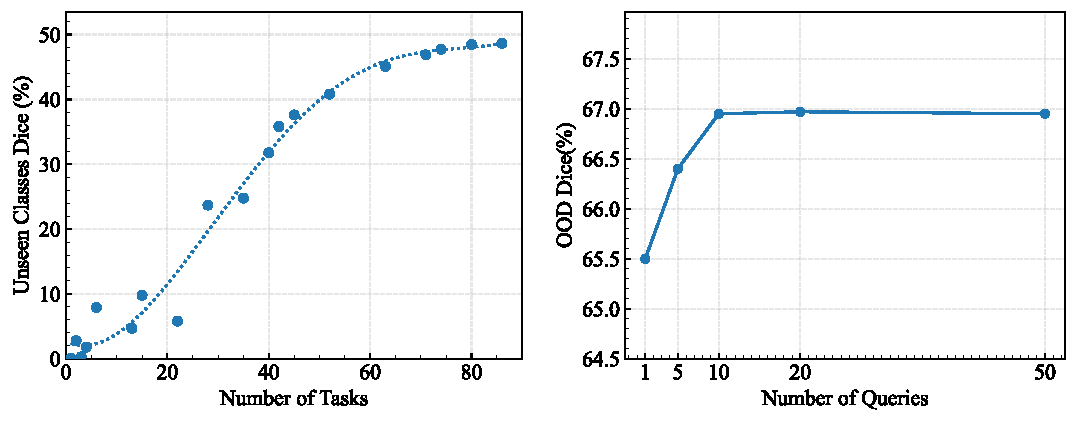
\includegraphics[width=\columnwidth]{./fig/ablation.pdf}
\end{center}
\vspace{-1em}
\caption{\textbf{Left}: Number of tasks used for training v.s. Performance on unseen classes. \textbf{Right}: Ablation on the number of queries. }
\label{fig:ablation}
\vspace{-1em}
\end{figure}




\begin{table}[t]
\centering
\caption{Ablation study of different components in Iris. High-Res: high-resolution feature processing; Foreground: foreground feature pooling; Query: query-based contextual encoding.}
\label{tab:ablation}
\resizebox{\columnwidth}{!}{
\begin{tabular}{cccccc}
\toprule
High-Res & Foreground & Query & In-dist (Avg) & In-dist (Small) & Out-of-dist \\
\midrule
         & \checkmark & \checkmark & 82.10 & 62.13 & 62.00 \\
\checkmark & \checkmark   & & 82.47 & 78.92 & 65.93 \\
\checkmark &  &\checkmark           & 82.06 & 77.53 & 64.13 \\
\rowcolor{lightgray}
\checkmark & \checkmark & \checkmark & \textbf{84.52} & \textbf{80.36} & \textbf{66.95} \\
\bottomrule
\end{tabular}
}
\vspace{-1em}
\end{table}






